\iffalse

\documentclass[12pt]{article}
\usepackage{graphicx}
\usepackage{amsmath}
\usepackage{mathtools}
\usepackage{gensymb}
\usepackage{tabularx}
\usepackage{array}
\usepackage[latin1]{inputenc}
\usepackage{fullpage}
\usepackage{color}
\usepackage{array}
\usepackage{longtable}
\usepackage{calc}
\usepackage{multirow}
\usepackage{hhline}
\usepackage{ifthen}
\usepackage{lscape}
\usepackage{float}
\usepackage{amssymb}

\newcommand{\mydet}[1]{\ensuremath{\begin{vmatrix}#1\end{vmatrix}}}
\providecommand{\brak}[1]{\ensuremath{\left(#1\right)}}
\providecommand{\cbrak}[1]{\ensuremath{\left\{#1\right\}}}
\providecommand{\norm}[1]{\left\lVert#1\right\rVert}
\providecommand{\abs}[1]{\left\vert#1\right\vert}
\newcommand{\solution}{\noindent \textbf{Solution: }}
\newcommand{\myvec}[1]{\ensuremath{\begin{pmatrix}#1\end{pmatrix}}}
\let\vec\mathbf

\def\inputGnumericTable{}

\begin{document}
\begin{center}
\textbf\large{OPTIMIZATION}

\end{center}
\section*{Excercise 10.3}


\solution
\fi
The given equation can be represented in parametric form as
\begin{align}
	\label{eq:11/10/3/3/2/grad/eq2}
	\vec{x} = \vec{A}+\lambda\vec{m}
\end{align}
where
\begin{align}
	\vec{A} = \myvec{2\\2}, \vec{m} = \myvec{1\\0}
	\label{eq:11/10/3/3/2/grad/line}
\end{align}
Let $\vec{O}$ be the origin. The perpendicular distance will be the minimum distance from $\vec{O}$ to the line. Let $\vec{P}$ be the foot of perpendicular. This problem can be formulated as an optimization problem as follows:
\begin{align}
	d_{\min} &= 	 \min_{\vec{x}}\norm{\vec{x}-\vec{O}}^2\\
	 &= \min_{\lambda}\norm{\vec{A}+\lambda\vec{m}-\vec{O}}^2\\
	&= \norm{\vec{m}}^2\lambda^2+2\lambda\vec{A}^\top\vec{m}+\norm{\vec{A}}^2
	\label{eq:11/10/3/3/2/grad/eq3}
	\\
	&= \lambda^2+4\lambda+8 = f^\prime\brak{\lambda} 
	\label{eq:11/10/3/3/2/grad/eq4}
\end{align}
upon substituting numerical values.
$\because$ the coefficient of $\lambda^2>0$, \eqref{eq:11/10/3/3/2/grad/eq3} is a convex function
The update equation using Gradient Descent is
\begin{align}
	\lambda_{n+1} &= \lambda_n - \alpha\nabla f\brak{\lambda_n}\\
	\label{eq:11/10/3/3/2/grad/eq5}
 &= \brak{1-2\alpha}\lambda_{n} - 4\alpha
\end{align}
Taking one-sided Z-transform on both sides of \eqref{eq:11/10/3/3/2/grad/eq5},
\begin{align}
	z\Lambda\brak{z} &= \brak{1-2\alpha}\Lambda\brak{z} - \frac{4\alpha}{1-z^{-1}}\\
	\Lambda\brak{z} &= -\frac{4\alpha z^{-1}}{\brak{1-\brak{1-2\alpha}z^{-1}}\brak{1-z^{-1}}}\\
	&= 2\brak{\frac{1}{\brak{1-\brak{1-2\alpha}z^{-1}}}-\frac{1}{1-z^{-1}}}\\
	\label{eq:11/10/3/3/2/grad/eq6}
	&= 2\sum_{k=0}^{\infty}\brak{\brak{1-2\alpha}^{k}-1}z^{-k}
\end{align}
from \eqref{eq:11/10/3/3/2/grad/eq6}, the ROC is
\begin{align}
	\abs{z}>\max\cbrak{{1,\abs{1-2\alpha}}}\\
	\implies 0<\abs{1-2\alpha}<1\\
	\label{eq:11/10/3/3/2/grad/eq7}
	\implies 0<\alpha<\frac{1}{2}
\end{align}
Thus, if $\alpha$ satisfies \eqref{eq:11/10/3/3/2/grad/eq7}, then from \eqref{eq:11/10/3/3/2/grad/eq6}
\begin{align}
	\lim_{n\to\infty} \lambda_{n} = -2
\end{align}
Choosing
\begin{enumerate}
\item $\alpha$ = 0.001
\item precision = 0.0000001
\item n = 10000000
\item $\lambda_0$ = 4
\begin{align}
	\lambda_{min} = -2
\end{align}
\end{enumerate}
\begin{align}
	\vec{x}_{min} &= \vec{P} = \myvec{2\\2}+\brak{-2}\myvec{1\\0}\\
	&= \myvec{0\\2}\\
	OP &= \norm{\vec{P}-\vec{O}}\\
	&= \norm{\myvec{0\\2}-\myvec{0\\0}}\\
	&= 2
\end{align}
See Fig. \ref{fig:11/10/3/3/2/grad/Fig1} and Fig. \ref{fig:11/10/3/3/2/grad/Fig2}
\begin{figure}[!h]
	\begin{center} 
	    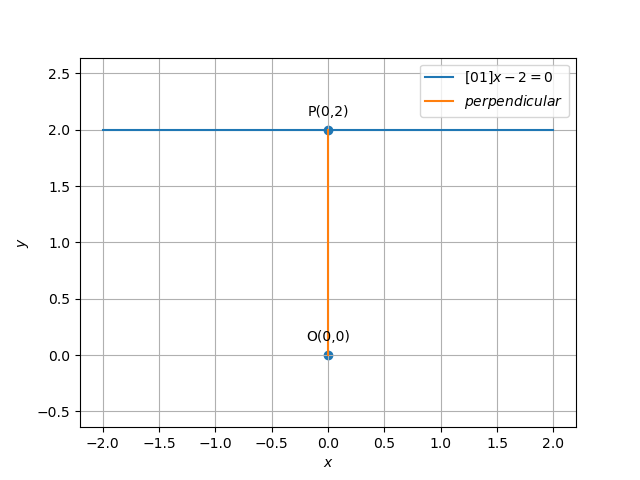
\includegraphics[width=\columnwidth]{11/10/3/3/2/grad/figs/opt1}
	\end{center}
\caption{}
\label{fig:11/10/3/3/2/grad/Fig1}
\end{figure}
\begin{figure}[!h]
	\begin{center} 
	    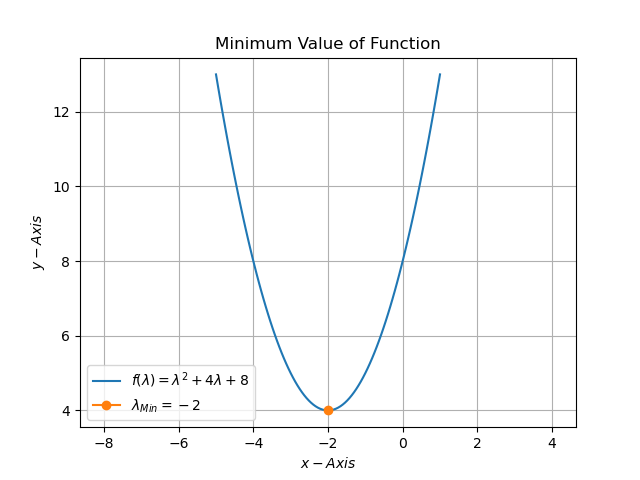
\includegraphics[width=\columnwidth]{11/10/3/3/2/grad/figs/opt2}
	\end{center}
\caption{}
\label{fig:11/10/3/3/2/grad/Fig2}
\end{figure}
